%!TEX root = ../thesis.tex
\chapter{Creating robust information flow measures}\label{ch:quotermodel}

The question underpinning this work is how information flows between news organisations. The cross entropy rate estimation introduced in \autoref{ch:crossentropy} is an important tool to tackle this challenge, but is not sufficient in isolation. To understand information flow in the news-media ecosystem we need a tool that meets three criteria: (1) it must accurately identify how much information flows between outlets, (2) it must determine the direction of that flow, and (3) it must do so in the presence of information noise.

In this chapter we examine the efficiency of the cross entropy rate as a tool for measuring information flow, and introduce new measures derived from it. These measures are tested in a variety of simulated conditions using both synthetic and real language data to determine the best approach for quantifying information flow.


\section{The quoter model}
The `quoter model'~\cite{bagrow_quoter_2018} is a simple model for capturing the dynamics of information flow on networks. This model places $N$ individuals in a network connected by directed edges. These edges indicate that a quoting process is occurring from the source of the edge, $j$, to the target, $i$. This network of quoting across edges is designed to mimic the information generation process of users on social media, where users create content by either adding new information to the platform, or copying/quoting information already seen in their feed.

Each edge is assigned a quote probability, $q_{ji}$, and each node has a self generation probability, $q_{ii}$. These probabilities are used to decide how a node behaves at each time step of a simulation and are normalised such that $\sum_{\forall i} q_{ij} = 1$. The model repeatedly performs a process of text generation for $T$ steps. At each time point $t$, every node creates text through one of two processes.

Starting from $t=0$, with probability $q_{ii}$ the node \emph{self generates} a new sequence of words with length $\lambda(t) \sim L(t)$. The probability distribution $L(t)$ can be any length distribution that is representative of natural text lengths. This can vary with $t$, but in in this work we exclusively use a Poisson distribution for all time steps $t$. Using this length $\lambda(t)$, the sequence of given length is generated by drawing from any distribution of words or sequences.  Each word in the generated sequence shares the same time step index $t$, which will become useful later when we want to draw only from the past of a node. These generated sequences and their associated time indices are concatenated into a single long timestamped sequence for each node.

Alternatively, at each time point from $t=1$ onwards the node can undergo a \emph{quote process}. With probability $q_{ji}$, the target can quote from a source, $j$, by selecting a point in the source's sequence uniform randomly. The source's sequence includes only words generated before time $t$. Starting from the selected point in the source's history, a subsequence of length $\lambda(t) \sim L(t)$ is copied from the source's history into the present of the target, and is added to the target's timestamped sequence with time $t$.

Importantly, the quote process draws from the source's past indiscriminately, and could copy a sequence of text that the source had previous quoted from elsewhere. This sequence itself could originally have been generated by the target, and arrived in the source's history though a series of random quoting rounds. 

In general, this results in a system of information being passed between the nodes in the network, dependent of the quoting probabilities over the edges.

The \emph{self generation} process can use any arbitrary method for generating a sequence given a length $\lambda(t)$. In the case of the original model~\cite{bagrow_quoter_2018}, two methods are used; drawing uniformly from a fixed vocabulary and drawing from a rank ordered vocabulary according to a Zipf distribution. In line with the previous chapter we use a Zipf distribution to generate text here.


\subsection{Single flow estimation} 

Previous work~\cite{bagrow_quoter_2018} used the Kontoyiannis cross entropy rate to examine flow direction and quoting probability. This approach is reasonable, and deeply rooted in the quoter model construction. The quoter model produces sequences in the future of a quoter that exactly match the quoted source. It is these sequences which the match-length based cross entropy rate measure captures. However, this approach can break down when the producers of text have non-homogeneous text production methods.

We can see where this assumption of homogeneous generation is violated by performing a simple experiment. We take two text-producing nodes and connect them by a single edge, as in \autoref{fig:fixedalphasingleflow}(b). The node $S$ will always produce new text, without ever quoting. The node $T$ will follow the simple quoter model rules, producing new text of length $\lambda \sim Poisson(3)$ with probability $1-q$ or quoting a length $\lambda$ from the history of the node $S$ with probability $q$. This link is simulated for a range of values for $q$ from 0 to 1. Both of these producers create their text by drawing from a Zipf distribution with scaling parameter~$\alpha=1.5$.

\begin{figure}[!htbp]
\centering
\includestandalone[width=\textwidth]{chapter3/figs/tikz/fixedalphasingleflow}
\caption{Simulations with node $S$ generating text from a Zipf distribution with scaling parameter $\alpha=1.5$ and node $T$ generating similarly with probability $1-q$ or quoting from $S$ with probability $q$. While the cross entropy rate is tightly correlated with $q$ (a), so two is the vocabulary size of $T$ (c) and the self entropy rate of $T$ (d). Simple linear models demonstrate that these comparison-free measures in (c) and (d) capture almost the same amount of explanatory information of $q$ as the cross entropy.}\label{fig:fixedalphasingleflow}
\end{figure}

We calculate the cross entropies between the two nodes in both directions, and other properties such as the entropy rate and vocabulary size of both $S$ and $T$ in isolation.

We perform separate linear regressions on the quoting probability for each of the properties, $\hat{h}(T||S)$, $\hat{h}(T)$ and the vocabulary. The properties and $q$ are transformed to a standard normal, with the logarithm of the vocabulary first being taken.
As expected, the cross entropy, $\hat{h}(T||S)$ and $q$ have a significant negative linear relationship ($p<10^{-15}$), with 99.6\% of the variance explained. This result seems positive, but needs to be addressed in context. The cross entropy does show the relationship between the two sources, but is also influenced by the sequence properties of $T$.

A fitted linear model between the self entropy rate $\hat{h}(T)$ and $q$ has a similar powerful negative linear relationship ($p<10^{-13}$, $R^2 = 0.886$). This result is a direct consequence of an important caveat of this model: it is sensitive to the vocabulary sizes of quote distributions. Indeed, the linear relationship between the normalised logged vocabulary of $T$ and the quote probability, $q$, shares the same predictive power ($p<10^{-13}$, $R^2 = 0.942$). This suggests that much of the predictive power in the cross entropy and self entropy rate is provided by the differences in vocabulary size between source and target. Hence, we first need to examine the distributions of vocabulary size under quoting regimes before we can move on.

\subsubsection{Vocabulary sizes of quoted distributions}
% https://math.stackexchange.com/questions/32800/probability-distribution-of-coverage-of-a-set-after-x-independently-randomly/32816#32816
% https://math.stackexchange.com/questions/227556/the-exact-probability-of-observing-x-unique-elements-after-sampling-with-repla/1957820#1957820
This tight relationship between vocabulary size and quoting probabilities can be explained by sampling from a distribution with replacement. 
\begin{theorem}
Suppose we have a set of tokens $S$ with a fixed finite vocabulary size $V_S$. If we take a sample with replacement of size $N$ from $S$, this sample $T$ has a random vocabulary size $V_T$, according to the distribution,
$$P(V_T = v) = \frac{S_{2}(N, v) V_S!}{V_S^{N}(V_S-v)!},$$
where $S_2(\cdot, \cdot)$ is the Stirling number of the second kind~\cite{graham_concrete_1989}.
\end{theorem}
\begin{proof} %{of the vocabulary after sampling with replacement}
The vocabulary size is given by the number of unique elements in the sample. For a sample with vocabulary size $v$, each element must come from the set of size $V_S$. Hence, the number of possible vocabulary sets of size $V_T$ is $\binom{V_S}{v}$.


Given a sample vocabulary set (which has size $v$), we must choose how the elements that we draw are distributed amongst that vocabulary set. In essence, we have a set of $v$ bins that we can fill with our $N$ elements in our sample. Rephrased, we are finding the number of ways to partition $N$ elements into $v$ labelled sets, which is given by, $v! S_2(N, v).$


Together, this gives that the total number of possible samples with vocabulary size $v$ is,
$$ \binom{V_S}{v} v! S_2(N, v) =  \frac{ v! S_2(N, v) V_S! }{(V_S - v)! v!} = \frac{S_2(N, v) V_S! }{(V_S - v)!}.$$

Finally, we must divide by the total number of possible samples, $V_S^N$, which gives,
$$P(V_T = v) = \frac{S_{2}(N, v) V_S!}{V_S^{N}(V_S-v)!}.$$
\end{proof}


From this we find that the expected value for $V_T$ is,
$$E\left[V_T \right] = V_S\left(1-\left(1-\frac{1}{V_S}\right)^{N}\right) < V_S.$$ 

This highlights an important point, that when taking a finite sample with replacement, the expected vocabulary size of the sample will be \emph{lower} than the source.

This is a useful upper bound on the expectation of our quoter vocabularies. We expect the quoter model vocabularies sizes to be smaller again, due to the finite size of the text data during quoting. At early stages of the simulations, very little text exists in the source, and hence $V_S$ will be very small to start with. This means that under very high quote probabilities, $V_S$ must grow before $V_T$ can grow. 

We can see this result in \autoref{fig:vocabsizes}. Two nodes are again simulated with a single flow edge between then as per \autoref{fig:fixedalphasingleflow}. When there is no quoting between the nodes ($q=0$), meaning they both draw words identically and independently using the self generation process, the nodes have almost identical vocabulary distributions. The nodes are simulated 10,000 times for 1000 time steps of generation, giving a mean vocabulary size of 415 for both. However, when $q=1$ the target node is exclusively quoting from the source and does not produce text of its own. As expected from the above result, we see a significantly left-shifted vocabulary distribution, with the target node having a mean vocabulary size of 240. \autoref{fig:vocabsizes} reveals that this shift in vocabulary size change under increase $q$ is smooth, by running 10,000 simulations with $q \sim U(0,1)$.

\begin{figure}[!htbp]
\centering
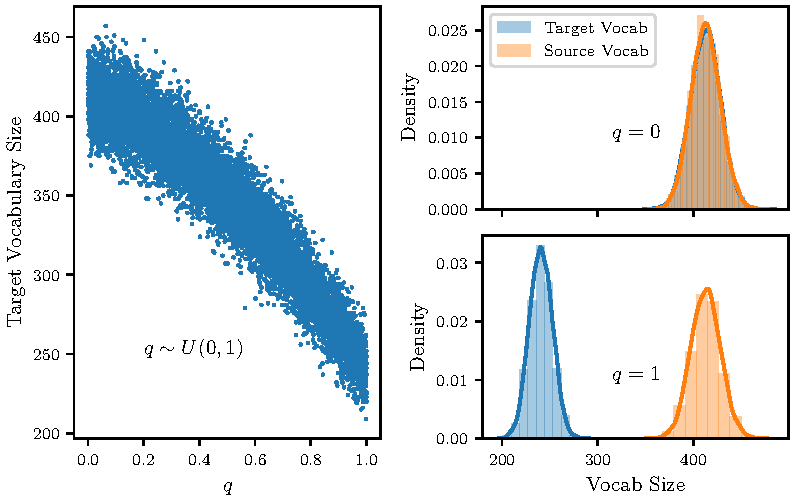
\includegraphics{chapter3/figs/VocabChangePlot.pdf}
\caption{A source produces text from a Zipf distribution of words. A target produces text similarly with probability $1-q$ or quotes from the source with probability $q$. The vocabulary size of the source and target are calculated by taking the number of unique elements after 1000 time steps. The vocabulary size of the target decreases as $q$ increases.}\label{fig:vocabsizes}
\end{figure}

\subsubsection{Variable vocabularies}
We next validate the ability of a measure to detect information flow beyond quoting. To achieve this, we introduce an extra dimension of variability to the model. 

Once again we have two text producers $S$ and $T$, shown in \autoref{fig:quoter_variable_vocab_tikz}, where $T$ quotes from $S$ with probability $q$. The source $S$ still creates text via a Zipf law distribution with scaling parameter $\alpha_S=1.5$, but the target $T$ now generates its own text at $\alpha_T \sim U(1.25,1.75)$, which is set at node creation. Having a larger scaling parameter will result in a smaller vocabulary distribution and \emph{vice versa}. This creates an interesting challenge for our measure. It needs to both account for the quoting along the edge, as well as natural variations in the text generation of $T$.

\begin{figure}[!htbp]
\centering
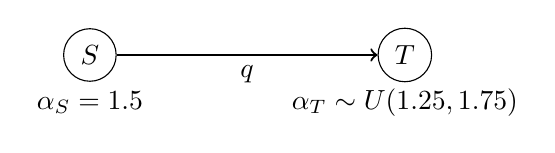
\begin{tikzpicture}[scale=2]
\node [draw, circle] (s) at (0, 0) {$S$};
\node [draw, circle] (t) at (2,0) {$T$}
edge [thick, <-] node[auto] {$q$} (s);

\node at (0,-0.3) {$\alpha_S = 1.5$};
\node at (2,-0.3) {$\alpha_T \sim U(1.25, 1.75)$};
\end{tikzpicture}
\caption{An diagram of a new quoting simulation regime. The target, $T$, now has a variable Zipf distribution scaling parameter for self generation, adding variability to the vocabulary size of its own self generated text.}\label{fig:quoter_variable_vocab_tikz}
\end{figure}

The single flow experiment run with these new generation protocols has vastly different results. \autoref{fig:flow_variablealphascatterplot} shows that the simulations with very low quoting probabilities exhibit high variance in the vocabulary size, which is directly attributable to the choice of $\alpha_T$. As the quoting probability approaches 1, the amount of self generation of text by $T$ reduces, resulting in a vocabulary of slightly under 66\% of the $S$ vocabulary size, as expected.


\begin{figure}[!htbp]
\centering
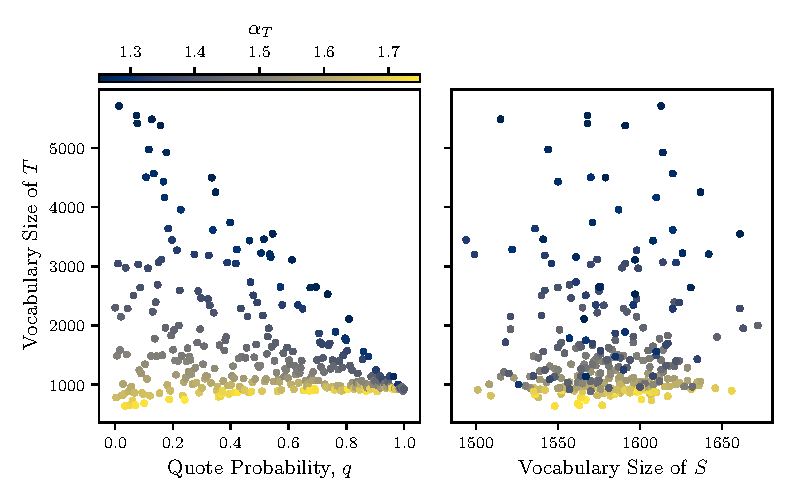
\includegraphics{chapter3/figs/VariableAlphaVocabSize.pdf}
\caption{The target node $T$ self generates with probability $1-q$ from a Zipf distribution according to a variable scaling parameter, $\alpha_T \sim U(1.25, 1.75)$. With probability $q$, $T$ quotes from the source, $S$, which always self generates with $\alpha_S = 1.5$. The added variability in the self generation at $T$ decouples the previous tight correlation between the vocabulary size and the self generation probability. }\label{fig:flow_variablealphascatterplot}
\end{figure}

Again a linear model is fitted on $q$ using $\hat{h}(T||S)$, with both variables being normalised. There is still a significant negative relationship ($p< 4\times10^{-6}$), but now with much less variance explained ($R^2 = 0.356$) compared to the previous experiment ($R^2=0.996$). In a similar fashion, both the self entropy rate and logged vocabulary size of $T$ have far lower explanatory power ($R^2=0.088$ and $R^2=0.163$ respectively).

Outside of simplified model conditions where text producers are identical, cross entropy rates are not themselves sufficient to identify the level of information flow. This is important as the real data discussed in \autoref{ch:data} has already been shown to have a wide range of vocabulary sizes. If only cross entropy rates were used on this data, the results would largely capture commonalities in vocabulary between pairs of organisations, and information flow measures would not be comparable. 

Performing a multiple linear regression on $q$ using a combination of variables provides a picture of how these variables relate. \autoref{tab:quoter_mutlipleOLS} shows models which combine $\hat{h}(T||S)$ with the opposite direction cross entropy, $\hat{h}(S||T)$, the self entropy rate of $T$, $\hat{h}(T)$, and the self entropy rate of $S$, $\hat{h}(S)$; with all variables being normalised. These models regressed on $q$ show a significant relationship with greater predictive power, hinting that more complex relationships between the metrics may be required to measures information across these edges. Indeed, in an environment where sources and targets have varying text generation parameters, such as in our real data, the use of other entropic estimates may be useful in controlling for these exogenous properties of the language. 

\begin{table}[!htbp]
\centering 
\begin{tabular}{c|rrrr}
Variable& Model 1& Model 2& Model 3& Model 4\\ \hline
$\hat{h}(S)$& & & & $-0.026^{**}\,\,$\\
$\hat{h}(T||S)$& $-0.444^{***}$& $-0.814^{***}$& $-0.641^{***}$& $-0.742^{***}$\\
$\hat{h}(T)$& & $0.679^{***}$& & $0.485^{***}$\\
$\hat{h}(S||T)$& $0.343^{***}$& & & $0.132^{***}$\\
Vocab($T$)& & & $0.490^{***}$& \\\hline
\rule{0pt}{3ex}$R^2$& 0.876\;\;\;\;& 0.966\;\;\;\;& 0.626\;\;\;\;& 0.979\;\;\;\;\\ \hline
\rule{0pt}{3ex}adj. $R^2$& 0.871\;\;\;\;& 0.965\;\;\;\;& 0.610\;\;\;\;& 0.977\;\;\;\;\\ \hline
\multicolumn{5}{c}{$p_{val}<0.1^*$, $p_{val}<0.01^{**}$, $p_{val}<0.001^{***}$} \\ \hline\end{tabular}
\caption{Four ordinary linear regressions are fit on $q$ using the entropy rates of $S$ and $T$, the cross entropy rates between $S$ and $T$ in both directions, and the vocabulary size of T, Vocab($T$). These variables are calculated from 1000 simulations of $T$ quoting $S$ with probability $q\sim U(0,1)$, or $T$ self generating using $\alpha_T\sim U(1.25, 1.75)$ with probability $1-q$. $S$ always self generates using $\alpha_S = 1.5$. These models suggest that a combination of variables can help predict $q$ when $T$ and $S$ have different generation distributions.} \label{tab:quoter_mutlipleOLS}
\end{table}


\section{Novel measures of information flow}

To better capture the true flow of information in a network, a more robust measure may be needed. Here we introduce several possible measures and test them in larger simulated networks.

Our first measure is the most naive. We simply take the difference between the cross entropy rates in both directions, 
\begin{equation}a_{\hat{h}}  = \hat{h}(T||S) - \hat{h}(S||T).\end{equation}
Remembering that the measure needs to identify both the direction and magnitude of the flow across the edge, $a_{\hat{h}} >0$ indicates a flow from $S$ to $T$, and the reverse from $T$ to $S$ if $a_{\hat{h}} <0$. Further, a good metric should be able to distinguish between edges with and without flow ($q=0$). This first measure can be seen as an `absolute' measure.

In contrast, the second and third measures, 
\begin{equation}
b_{\hat{h}} := \frac{\hat{h}(T||S)}{\hat{h}(S)} - \frac{\hat{h}(S||T)}{\hat{h}(T)},
\end{equation}
and
\begin{equation}
c_{\hat{h}} := \frac{\hat{h}(T||S)}{\hat{h}(T)} - \frac{\hat{h}(S||T)}{\hat{h}(S)},
\end{equation}
normalise the cross entropy rates by the self entropy rates of the source, in $b_{\hat{h}}$, and the target, in $c_{\hat{h}}$. In theory, these self entropy rates may help create a fair comparison between the cross entropy rates in each direction.

For example, if a source was to have an extremely large vocabulary, or otherwise have complex language leading to a high information content, the cross entropy rate would be naturally inflated regardless of the quoting probability. Normalisation by entropy rate may hence improve detection.

The final set of measures seek to solve the problem of entropy normalisation, as well as the challenges of increased complexity of quote dynamics (such as the presence of quote cycles and chains of quoting) posed by larger networks. The measures, 
\begin{equation} 
	d_{\hat{h}} := \frac{\hat{h}{(T||S)}}{\sum_X \hat{h}(X||S)} - \frac{\hat{h}(S||T)}{\sum_X \hat{h}(X||T)},
\end{equation} 
and
\begin{equation} 
	e_{\hat{h}} := \frac{\hat{h}(T||S)}{\sum_X \hat{h}(T||X)} - \frac{\hat{h}(S||T)}{\sum_X \hat{h}(S||X)},
\end{equation}
seek to normalise the cross entropy rates using local neighbourhood network information, by dividing by the average cross entropy out of the source ($d_{\hat{h}}$) or into the target ($e_{\hat{h}}$). 

This seeks to solve a deeper challenge, namely that in densely connected networks, there can be feedback loops and chains of information flow. Normalising using local network information may provide additional insight into the flow on single edges within the larger network.

So far we have discussed measures using only cross entropy rates and self entropy rates. For each metric we also consider the same measures with entropy rates $\hat{h}(T||S)$ replaced with predictabilities $\hat{\pi}(T||S)$. These predictabilities introduce a level of normalisation by the vocabulary of the target distribution. Greater flow likelihoods are represented by \emph{higher} predictabilities and \emph{lower} cross entropy rates; as such, the equations using $\hat{\pi}(T||S)$ are reversed in sign.

\autoref{tab:measures} shows the collection of all of the measures discussed here. 

\begin{table}[!htbp]
\centering
\begin{tabular}{cc}
 Entropy Based & Predictability Based  \\ 
\toprule
% \multirow{2}{*}{Naive}
 $ \displaystyle a_{\hat{h}} := \hat{h}(T||S) - \hat{h}(S||T)$ & 
$ \displaystyle a_{\hat{\pi}} := \hat{\pi}(S||T) - \hat{\pi}(T||S)$ \\
\midrule
% \multirow{2}{*}{Normalised}
 $ \displaystyle b_{\hat{h}} := \frac{\hat{h}(T||S)}{\hat{h}(S)} - \frac{\hat{h}(S||T)}{\hat{h}(T)}$ & 
$ \displaystyle b_{\hat{\pi}} := \frac{\hat{\pi}(S||T)}{\hat{\pi}(T)} - \frac{\hat{\pi}(T||S)}{\hat{\pi}(S)}$ \\
 $ \displaystyle c_{\hat{h}} := \frac{\hat{h}(T||S)}{\hat{h}(T)} - \frac{\hat{h}(S||T)}{\hat{h}(S)}$ & 
$ \displaystyle c_{\hat{\pi}} := \frac{\hat{\pi}(S||T)}{\hat{\pi}(S)} - \frac{\hat{\pi}(T||S)}{\hat{\pi}(T)}$ \\
\midrule 
% \multirow{2}{*}{Network}
 $ \displaystyle d_{\hat{h}} := \frac{\hat{h}(T||S)}{\sum_X \hat{h}(X||S)} - \frac{\hat{h}(S||T)}{\sum_X \hat{h}(X||T)}$ &
$ \displaystyle d_{\hat{\pi}} := \frac{\hat{\pi}(S||T)}{\sum_X \hat{\pi}(X||T)} - \frac{\hat{\pi}(T||S)}{\sum_X \hat{\pi}(X||S)}$  \\
\addlinespace[0.5ex]
 $ \displaystyle e_{\hat{h}} := \frac{\hat{h}(T||S)}{\sum_X \hat{h}(T||X)} - \frac{\hat{h}(S||T)}{\sum_X \hat{h}(S||X)}$ & 
$ \displaystyle e_{\hat{\pi}} := \frac{\hat{\pi}(S||T)}{\sum_X \hat{\pi}(S||X)} - \frac{\hat{\pi}(T||S)}{\sum_X \hat{\pi}(T||X)}$ \\
\end{tabular}
\caption{A glossary of the measures introduced to detect information flow.}\label{tab:measures}
\end{table}


\subsection{Network simulations}\label{sec:network_sizes}
To evaluate the quality of the information flow measures, we use quoter model simulations on larger networks to examine how the measures perform under various network types. 

In \autoref{fig:flow_networksize}, cliques are generated for sizes, $N=2$ to $N=50$. In the clique, each possible pair of nodes, $(j,i)$, is connected with a direction (bi-directional links are not allowed) and a preliminary edge quote probability, $q_{ji}' \sim U(0,1)$. Each node is assigned a self generation probability, $q_{ii}=0.5$. The incoming quote probabilities are normalised across the local incoming edges, 
$$q_{ji} = q_{ji}' / \left( \sum_{k\neq i} q_{ki}' + q_{ii} \right),$$
while the self generation probability is held constant. 

As above, the network undergoes a procedure of text generation wherein a node $i$ generates a new sequence of length $\lambda \sim Poisson(3)$ from a Zipf distribution with scaling parameter $\alpha = 1.5$ or quotes a $\lambda$ long subsequence from neighbour $j$ with probability $q_{ji}$.

This generation procedure is performed for 7000 time steps to produce a quoter model network with sequences averaging $7000\times\mathbb{E}[\lambda]=21,000$ tokens. As we saw in \autoref{ch:crossentropy}, this is a sufficient number of tokens to allow for cross entropy convergence while balancing speed of computation. Cross entropy rates are calculated between every pair of edges and self entropy rates are calculated for every node. We then compute the information flow measures in \autoref{tab:measures}. For each network size, $M$, simulations were repeated such that there were at least 500 edges being estimated (\emph{e.g.}, $M=2$ requires 500 simulations while $M=3$ requires 167), with a minimum number of 4 simulations (\emph{e.g.}, $M=49$ has 1176 edges to estimate, but is repeated 4 times for a total of 4704 data points). For each $M$, the Pearson correlation coefficient is calculated between the true quote probability and the estimated information flow using each measure.

\begin{figure}[!htbp]
	\centering
	\begin{subfigure}[t]{\textwidth}
		\centering
		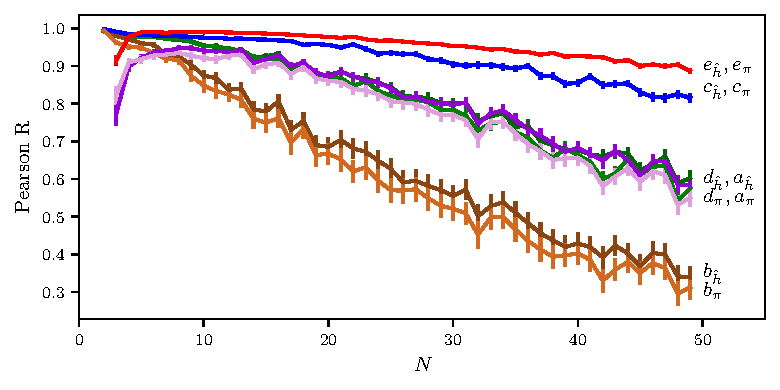
\includegraphics{chapter3/figs/zipf_network_size.pdf}
		\caption{Changing network size of random-orientation directed cliques.}
		\label{fig:flow_networksize}
	\end{subfigure}

	\begin{subfigure}[t]{\textwidth}
		\centering
		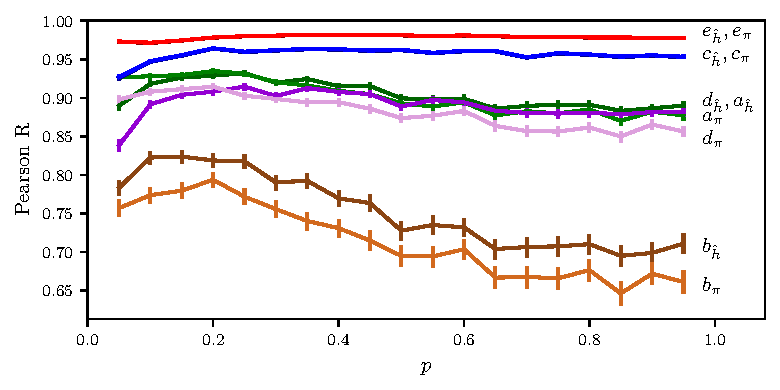
\includegraphics{chapter3/figs/zipf_ER.pdf}
		\caption{Changing edge probability of Erdős–Rényi networks.}
		\label{fig:flow_ERchange}
	\end{subfigure}
	\caption{Networks are generated from a quoter model with varying network size and edge probability. For each set of parameters 95\% confidence intervals are shown for the Pearson correlation between the true quote probability and the estimated information flow for each flow measure. (a) shows simulations on directed cliques with every pair of nodes having a directed single edge between them. Network size $N$ is varied, with larger networks resulting in smaller correlations. (b) takes an Erdős–Rényi network with 20 nodes and varying edge probability $p$. Flow correlations are consistent across $p$ for measures $e$ and $c$ despite increasing edge density while $b$ measures see a slight decline in performance. \label{fig:flow_sizeandER}}
\end{figure}

% Results
\autoref{fig:flow_networksize} shows that estimating quote probabilities typically becomes harder for larger network sizes. %
% This is expected as larger clique networks will have more self loops of quoting, and greater interdependence of text. 
Measures $e$ and $c$, which both normalise by the complexity of the target, outperform all others, with the local neighbourhood network information adding a slight improvement for $e$. These measure perform well using both cross entropy and cross predictability, with almost identical results which obscure the overlapping lines in the figure. Measures $a$ and $d$ perform equally well, with the predictability measures performing worse than the cross entropy measures. The tight relationship is surprising given that $a$ has no normalisation and $d$ normalises by the cross entropy / cross predictability into each source. Normalising by the source information proves counter productive, with $b$ have the lowest correlations between the true edge flows and estimated flows.

These trends are consistent as $N$ increases, with one caveat. For small $N$ ($\leq 5$) the local neighbourhood information based measures perform \emph{worse} than their non-network counterparts. % WHY?

A similar set of simulations is performed using a fixed size network ($N=20$) and directed edges generated randomly with probability $p$. Each edge in this Erdős–Rényi graph is assigned a quote probability and normalised exactly as above. All nodes self generate with a fixed probability $q_{ii}=0.5$. The general ranking of the measures remains consistent for all $p$ in \autoref{fig:flow_ERchange}. Measure $e$ consistently outperforms all other measures followed closely by measure $c$, this is likely as both measures $e$ and $c$ are normalising by the target complexity in both directions, with the network information giving a slight advantage to $e$. The rankings of measures $a$ and $d$ have similar Pearson correlation coefficients and remain close throughout. 

This increasing edge probability $p$ also corresponds to an increasing network density. Interestingly, one may expect that an increase in network density would make information flow estimation more difficult as more triangles are closed into cycles and confounding triplets. This is especially surprising given increases numbers of edges will result in a lower quote probability when outgoing quote probabilities are normalised. The ability for the $e$ measures to successfully estimate the information flow under these increasingly difficult conditions is impressive. 

It is useful to remember that the Erdős–Rényi graph with $p=1$ is identical to the graph generation at point $N=20$ above. This approach will help us with the next question, disentangling the effect of edge quote probability and network complexity.   

\subsection{Disentangling complexity from quote probabilities}\label{sec:low_quote_probs}
% disentangling complexity vs low quote probabilities
With increasing network sizes comes both increasing conversational complexity and lower individual quote probabilities. This conversational complexity simply comes from having more nodes quoting each other. Whenever a quoting cycle appears (A quotes B; B quotes C; C quotes T) we could expect for difficulty in measuring the flow across individual edges, as the signal between the three would become mixed. As network size increases in a clique graph, more of these cycles appear.  

In addition to this, the increasing network size lowers the quote probabilities across each individual edge. As a directed clique graph with a single edge between each pair of node, each node will have an average of $(N-1)/2$ neighbours to quote from. Since the self generation probability is fixed at $q_{ii}=0.5$, the remaining neighbours must share the leftover probability between them. This results in lower quote probabilities across the edges, which provide less signal making them harder to detect amongst the noise. Hence, it is harder to estimate small quote probabilities.

\autoref{fig:flow_quote_scatterplot} shows these quote probability differences by comparing measures $a_{\hat{h}}$ and $e_{\hat{h}}$ against the edge quote probabilities ($q_{ij}$) from networks of size $N=8$ and $N=30$. The quote probability has a much larger range of [0,0.5] for the smaller $N=8$, with a smaller range [0, 0.14] for $N=30$.

The variance in the measures for low quote probabilities is very similar at both network sizes, however, the high quote probabilities of the small network add leverage to the Pearson correlation. In essence, we can view the underlying variance in flow estimates as a property of the language complexity. Sub-sequences of text can repeat themselves independently in different generators when both draw from the same or similar distributions. This noise is a property of the self generation process, not the quoting process. Given the fixed self generation probability, this aspect of variance is constant regardless of the quote probabilities. Indeed, when a no-intercept linear regression is performed for each $N$, the residuals exhibit homoscedasticity across the range of true quote probabilities and the standard deviation of the residuals is similar across all $N$ (95\% CI of $\sigma_{residuals}$: [0.186, 0.228]). 

Having high individual edge quote probabilities allows for the signal of those flows to be picked up through the noise, and leads to a stronger tail of high flow and high quote probability points. This naturally increases the Pearson correlation coefficient.

A common solution to high leverage points is to use a Spearman correlation coefficient, which uses ranks rather than values. However in this problem the Spearman correlation provides almost identical values to the Pearson. The higher value points are not outliers, but rather the tail end of a well-spread distribution across the [0,0.5] range, and low rank words still experience the same signal-noise trade-off as when comparing Pearson correlations for different distributions of edge quote probabilities.


\begin{figure}[!htbp]
	\centering
	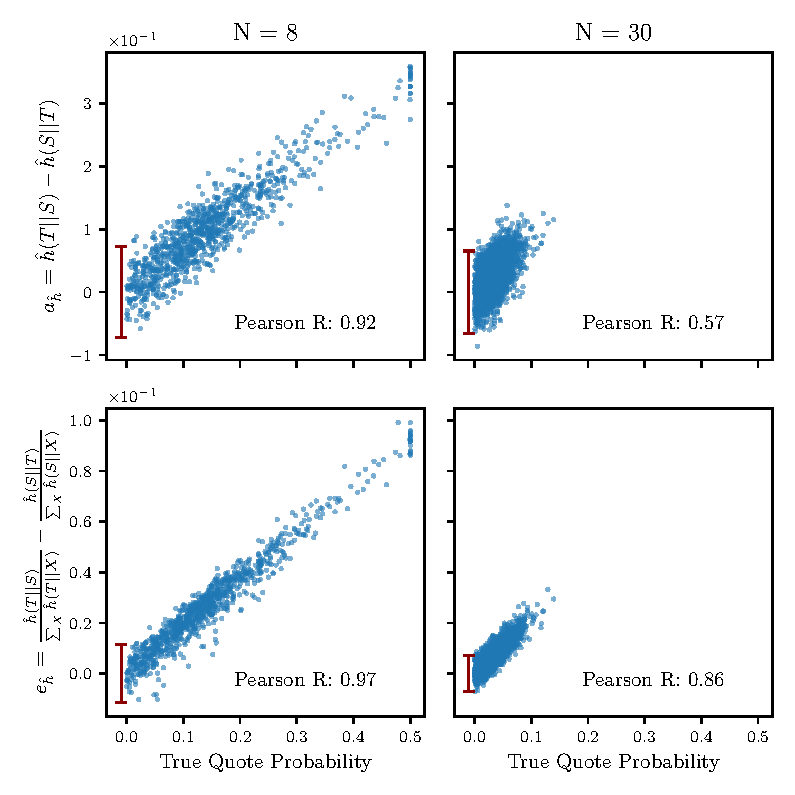
\includegraphics{chapter3/figs/scatterplot_comparison.pdf}
	\caption{Examples relationships between the true quote probability on a link between two notes and an information flow metric. Simple difference metrics such as $a_{\hat{h}}$ perform well on smaller networks with few nodes (N=3), but larger networks (N=30) need local neighbourhood information to perform well. For small networks, the tail high end quote probabilities pull up the Pearson correlation as they have stronger signal to overcome the constant variance from natural language generation. The {\color{red!40!black}dark red} bar shows the width of the 99\% confidence interval for the residuals of a no-intercept linear regression.}
	\label{fig:flow_quote_scatterplot}
\end{figure}

To further verify this effect we can vary the previous fixed self generation probability. As before, the edge quote probabilities normalise such that all generation and quote probabilities sum to one. Increasing $q_{ii}$ thus has the effect of shrinking these edge quote probabilities $q_{ji}$. If the above logic holds, then we would expect the increasing $q_{ii}$ values to decrease the Pearson correlation between $q_{ji}$ and the estimated flow. Indeed, in \autoref{fig:flow_self_p_vs_pearson_R} this pattern is observed with a clear decline in performance for all measures as the self generation probability increases. 


\begin{figure}[!htbp]
	\centering
	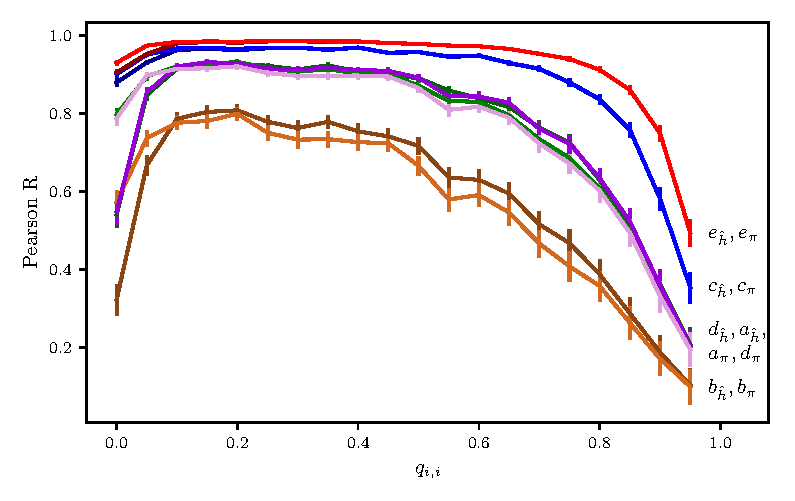
\includegraphics{chapter3/figs/zipf_self_p.pdf}
	\caption{Clique networks with 20 nodes are generated with each edge being assigned a direction and an edge quote probability $q_{ji}'$. The edge quote probabilities are added to the fixed self generation probability $q_{ii}$ and normalised. Increasing $q_{ii}$ decreases the edge quote probabilities on average which in turn decreases the Pearson correlation between the edge quote probabilities and the measured information flow. When no self generation is present ($q_{ii}=0$) only the generation seeds from $t=0$ are propagated, reducing measure performance.}
	\label{fig:flow_self_p_vs_pearson_R}
\end{figure}

Notably, there is also a decline in correlation at $q_{ii}=0$. In such a scenario the model would have all nodes quoting from one another based solely on the initial self generation step that seeds the process. This is surprising that even in an environment where limited source material exists, the measures still perform reasonably robustly.

\subsection{The effect of rewiring on measure performance}
In \autoref{sec:network_sizes}, we observed that increasing network size reduced the performance of information flow measures. \autoref{sec:low_quote_probs} showed that this is, in part, due to decreasing individual edge quote probabilities. However, increasing network size also increases the number of edges into and out-off each node. This leads to more cycles within the graph (even if they are of lower weights), making it difficult to determine sources of information. 

To isolate the effect of the network complexity on measure performance, we introduce a new simulated network. The Watts–Strogatz random graph model~\cite{watts_collective_1998} is used with a rewriting parameter $\beta$. In the model a graph is generated as a lattice, where each node in a network of size 20 is connected to its 8 nearest neighbours. These edges are assigned a random direction and weight, similar to the network models above. With probability $\beta$, the endpoint of each edge will rewire to attach to a random node. As $\beta$ increases, the network becomes less structured and more chaotic, with the clustering coefficient decreasing from its initial value of 0.64. In \autoref{fig:flow_zipf_watts_strogatz_model} these networks are generated for values of $\beta$ and the correlation coefficients are calculated for each measure. No trend is observed between $\beta$ and the correlation, indicating that the structural complexity of the network has no effect on measure performance when the distribution of individual quote probabilities are fixed. 

\begin{figure}[!htbp]
	\centering
	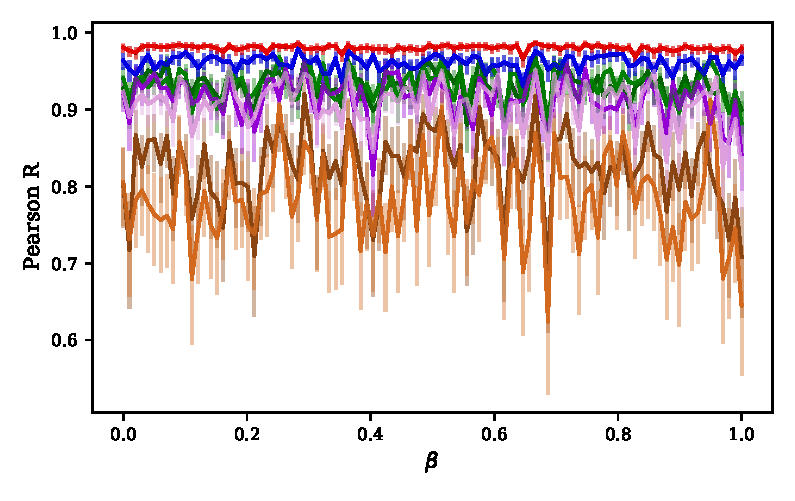
\includegraphics{chapter3/figs/zipf_watts_strogatz.pdf}
	\caption{A Watts–Strogatz random graph is generated with $N=20$ nodes and each edge assigned a direction and quote probability. These edges rewire with probability $\beta$. Information flow measures perform at consistent levels for all values of $\beta$, indicating that changing network structure has no impact on measure performance. 
	High variance in correlation is seen for measure {\color{brown}$b$ (brown)} with medium variance in {\color{violet}$d$ (purple)} and {\color{green!80!black}$a$ (green)}. This variance is exemplified by the large confidence intervals on the Pearson correlation coefficient which stands in contrast to the tight confidence intervals and low variance of measures {\color{red}$e$ (red)} and {\color{blue!80!black}$c$ (blue)}.}
	\label{fig:flow_zipf_watts_strogatz_model}
\end{figure}

This leads to the conclusion: the ability of the measures to correctly identify information flow is mostly dependent on the strength of the underlying quote probabilities to overcome the inherent noise present in text. While this conclusion is clear from the above results, they have used a simulated language model using Zipf distributions rather than real natural language. In order to confirm these results real data must be incorporated.


\section{Incorporating properties of real data}
A key limitation of the quoter model is the lack of foundation in real text data. Word generation processes such as those based on Zipf law are indeed derived from the analysis real data, but fall short of generating text that appears natural in most senses. The words generated using this method are independent, and lack the coherent structure of English grammar.

To rectify this, we update the \emph{self generation} process to use real text data. Using the corpus of Twitter data for news sources, each node in a simulated quoter graph is assigned a single news source. At each time step of the simulation a node can self generate by drawing a single random tweet from the entire history of the chosen outlets tweets and appending it to the node's timestamped sequence. The quoting process is identical, with each quote now drawing on sequences made from real tweets. Each simulation is run for 8000 time steps to maintain a consistent average sequence length. 

Since the average number of tweets for each news outlets is 19,337, drawing uniformly randomly with replacement would result in 33.9\% of tweets being drawn multiple times. To quickly prove this, assume we can draw a single tweet from $m$ tweets with probability $\frac{1}{m}$. The distribution of the number of times we draw that tweet over $X$ draws is $Binomial(X, \frac{1}{m})$, giving the cumulative probability that we draw it greater than one time being $1-\binom{X}{1} \frac{1}{m}(1-\frac{1}{m})^{X-1} - \binom{X}{0} (1-\frac{1}{m})^X = 1- Xp(1-\frac{1}{m})^{X-1} - (1-\frac{1}{m})^X$. With $m=19,337$ and $X=8,000$ this gives 0.338783. To rectify this, tweets are drawn without replacement. 

\begin{figure}[!htbp]
	\centering
	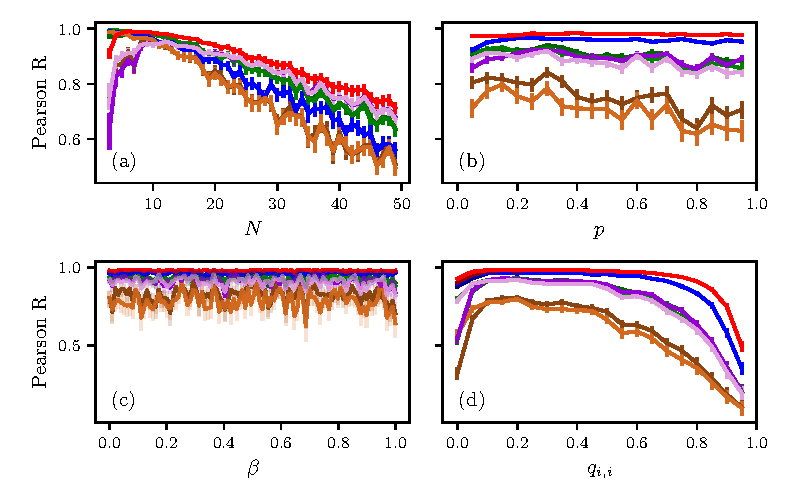
\includegraphics{./chapter3/figs/real_data_simulations.pdf}
	\caption{Networks are generated with $N$ nodes where each pair of nodes has an directed edge that exists with probability $p$ and is assigned a quote probability $q_{ji}'$. These quote probabilities are normalised such that their sum added to the fixed self generation probability, $q_{ii}$ equals 1. This self generation process draws from the Twitter history of a news outlet which is assign at network creation. (b), (c) and (d) use $N=20$ while (a) varies $N$. (a), (b) and (c) use $q_{ii}=0.5$ while (d) varies $q_{ii}$.  (a) and (d) use $p=1$ while (b) varies $p$ and (c) uses a more sophisticated Watt-Strogatz model which starts as a lattice with $p=0.4$ and requires edge endpoints with probability $\beta$. All simulations using real data for text generation follow the same results as their counterpart experiments using Zipf distributions for text generation.}
	\label{fig:flow_realdataquotermodel}
\end{figure}

Using this new self generation process the same experiments are run as above. \autoref{fig:flow_realdataquotermodel} combines the results from \autoref{fig:flow_sizeandER}, \autoref{fig:flow_self_p_vs_pearson_R} and \autoref{fig:flow_zipf_watts_strogatz_model}, updated to use real data. The core results outlined above remain exactly the same when using real data in place of simulated text in the model. 


\section{Go with the flow: applying the information flow measure}\label{sec:gowiththeflow}
\subsubsection{Selecting the best measure}
Put together, the results in this chapter suggest two key findings; the cross entropy is not a sufficient measure of information flow without normalising by the target entropy properties; and the information contained in the local neighbourhood structure is more informative than the entropy rate of a target alone.

Throughout every comparison done here the ranking of the measures fall into four categories.
\begin{itemize}
\item Measures $e_{\hat{h}}$ and $e_{\hat{\pi}}$ consistently outperform all other measures for networks of size greater than 5. These measures work by normalising the cross entropy or cross predictability using the local neighbourhood cross entropies or cross predictabilities going into the \emph{target}. While both types of the measure perform equally well in the large networks, the measure under-performs for networks with less than 5 nodes, as expected given the limited neighbourhood information.

\item Measures $c_{\hat{h}}$ and $c_{\hat{\pi}}$ perform slightly worse than the $e$ measures in large networks, but still hold their own. These measures work by normalising by the entropy or predictability of the \emph{target} without any knowledge of the network structure. Indeed, the lack of required network information allows this measure to perform the best for very small networks.

\item Measures $a_{\hat{h}}$,  $a_{\hat{\pi}}$, $d_{\hat{h}}$ and $d_{\hat{\pi}}$ perform consistently poorly when quote probabilities become low. The similarity between these measures is somewhat surprising given that $a$ has no normalisation while $d$ normalises by the local neighbourhood of the \emph{source}; indicating that the source neighbourhood provides almost no value to the calculation of flow.

\item Measures $b_{\hat{h}}$ and $b_{\hat{\pi}}$ which normalise by the entropy rate or predictability of the source without network information perform even worse than the simple difference between un-normalised cross entropies. 
\end{itemize}

From these results we find that $e_{\hat{h}}$ and $e_{\hat{\pi}}$ are the best measures. While either measure would be suitable in synthetic conditions, we choose to use $e_{\hat{\pi}}$ as we apply the measure to real data. In the simulations throughout this chapter we have seen the impact of vocabulary size on the measurement of information flow. As the real variety of text produces vary in vocabulary by an order of magnitude, we use the predictability version to help further counteract the impact of the vocabulary. 

Hence, we move forward using the measure,
\begin{equation} 
e_{\hat{\pi}} := \frac{\hat{\pi}(S||T)}{\sum_X \hat{\pi}(S||X)} - \frac{\hat{\pi}(T||S)}{\sum_X \hat{\pi}(T||X)}
\end{equation}
as the most robust tool to estimate information flows in networks of natural language text. 

\subsubsection{Results of applying the best measure}

Using measure $e_{\hat{\pi}}$ we can perform estimates of information flow between each pair of news organisations. In \autoref{sec:running_estimations} we performed the estimation of the entropy rates and cross entropy rates between all pairs of organisations using the entire corpus of tweets by each organisation for the 2019 calender year. Once these estimates are calculated, applying the information flow measure is computationally simple final step to extracting the estimates of flow. \autoref{fig:flow_appliedtodata} shows the distribution of these estimates for all pairs of organisations. As $e_{\hat{\pi}}$ is symmetrical around 0 when you swap the source and target, we choose the positive flow as the direction of the edge and assign its weight to be the flow estimate.

% \begin{figure}[!htbp]
% 	\centering
% 	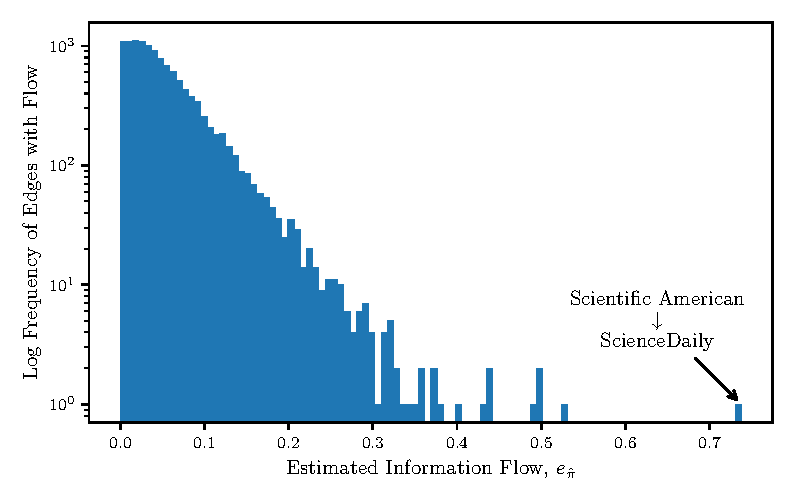
\includegraphics{./chapter3/figs/edge_weights.pdf}
% 	\caption{Information flow is estimated using measure $e_{\hat{\pi}}$ between each pair of news-media organisations using their entire tweet corpus. Each edge is assigned a direction and the positive weights of those edges are shown here. Most edges show very little information flows with only 1.6\% of edges having a flow estimate above 0.2. }
% 	\label{fig:flow_appliedtodata}
% \end{figure}

\begin{figure}[!htbp]
	\centering
	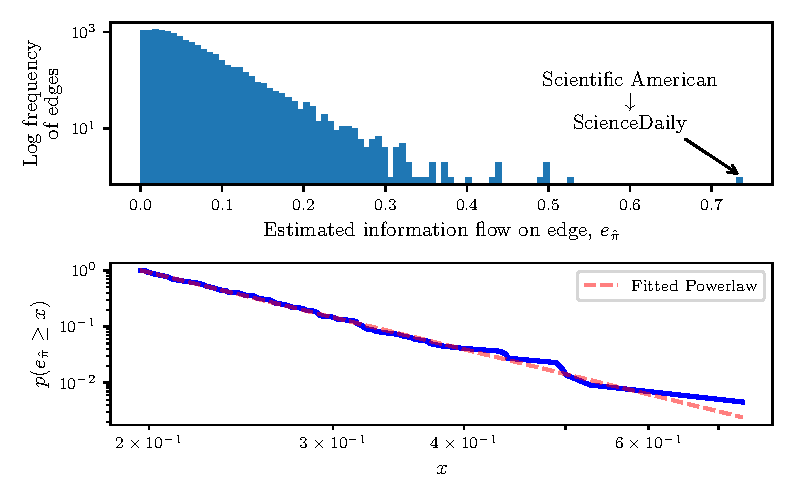
\includegraphics{./chapter3/figs/edge_weights_ccdf.pdf}
	\caption{Information flow is estimated using measure $e_{\hat{\pi}}$ between each pair of news-media organisations using their entire tweet corpus. Each edge is assigned a direction and the positive weights of those edges are shown. Most edges show very little information flows with only 1.6\% of edges having a flow estimate above 0.2. A complementary cumulative distribution function is shown with a fitted power law with exponent 5.6. }
	\label{fig:flow_appliedtodata}
\end{figure}

It is important to note that these flow estimates are not directly measuring a proportion of tweets that are copied, but rather a relative measure of how much informational content of the source is present in the target, compared to other pairs of organisations. 

Two key features of \autoref{fig:flow_appliedtodata} stand out: the heavy right skew of the distribution and the few outliers. Of the edges weight, 98.4\% are less that 0.2 leaving only 199 edges with weight greater than 0.2. This is important to note as \autoref{sec:low_quote_probs} highlighted that flow estimates are harder to disentangle from the noise of natural language when the information flow is low. Much of the flow estimate edges may be detecting a weak flow purely due to the commonality of their natural language. 

Noting the challenge created by information noise, these flow edges are useful for two purposes: comparing the magnitude of flows between two different pairs, and identifying the direction of flow when the flow estimate is large enough. As an example of the first, we can find that, as an information source, the \emph{New York Times} has relatively little net information flow to the \emph{Washington Post} (0.0053) but relatively high net information flow to the \emph{Foreign Affairs Magazine} (0.1480).

As an example of the second purpose, we examine the highest flow edge in the network, from the \emph{Scientific American} to \emph{ScienceDaily}.  This edge with weight (0.7378) is likely due to a confounding of factors. Firstly, \emph{Scientific American} is a popular and well resourced organisation that produces a large volume of content. The smaller and less popular \emph{ScienceDaily} is unlikely to get the `scoop' on many scientific stories meaning most content it posts will exist in the history of \emph{Scientific American}. Finally, \emph{ScienceDaily} has the least tweets, tokens and second least vocabulary of any organisation. This makes the normalisation of the information flows difficult due to its vocabulary being at the extreme of the distribution. 

In constructing these weighted edges into a network, it would be ideal to filter out low flow edges to make the graph more sparse for analysis. However, choosing such a cut-off is dubious at best and the power law distribution of estimated information flows has no natural scale at which to truncate. 

In the next chapter we explore several methods of using this network to rank the net information influence of news-media organisations and examine the inconsistency in their results.

